% !TEX TS-program = pdflatex
% !TEX root = tesi.tex

\documentclass[
  a4paper,
  twoside,
  openright,
  titlepage,
  headinclude,
  footinclude,
  BCOR5mm,
  numbers=noenddot,
  cleardoublepage=empty,
  tablecaptionabove
]{scrreprt}

\usepackage[T1]{fontenc}
\usepackage[utf8]{inputenc}
\usepackage[english]{babel}
\usepackage{amsmath}
\usepackage{amssymb}
\usepackage{indentfirst}
\usepackage[
  style=philosophy-modern,
  hyperref
]{biblatex}
\usepackage{chngpage}
\usepackage{calc}
\usepackage{listings}
\usepackage{graphicx}
\usepackage{subfig}
\usepackage{lipsum}
\usepackage{shapepar}
\usepackage{pifont}
\usepackage[
  eulerchapternumbers,
  subfig,
  beramono,
  eulermath,
  pdfspacing,
  listings
]{classicthesis}
\usepackage{arsclassica}
\usepackage{tikz}

% FONT UTILIZZATO DAL CONSERVATORIO
\usepackage[defaultfam,tabular,lining]{montserrat} %% Option 'defaultfam'
%% only if the base font of the document is to be sans serif
\usepackage[T1]{fontenc}
\renewcommand*\oldstylenums[1]{{\fontfamily{Montserrat-TOsF}\selectfont #1}}

\usepackage{ccicons}

% ********************************************************************
% Personal commands
% ********************************************************************
\DeclareRobustCommand*{\clsname}[1]{{\normalfont\sffamily#1}}
\DeclareRobustCommand*{\pkgname}[1]{{\normalfont\sffamily#1}}
\DeclareRobustCommand*{\optname}[1]{{\normalfont\ttfamily#1}}
\DeclareRobustCommand*{\cmdname}[1]{\mbox{\lstinline[basicstyle=\normalsize\ttfamily]!\\#1!}}

\DeclareRobustCommand*{\classicthesis}{Classic\-Thesis}
\DeclareRobustCommand*{\arsclassica}{{\normalfont\sffamily ArsClassica}}

% ********************************************************************
% Hyper-references
% ********************************************************************
\newcommand{\mail}[1]{\href{mailto:#1}{\texttt{#1}}}


% ********************************************************************
% Graphics
% ********************************************************************
\graphicspath{{Graphics/}}


% ********************************************************************
% Code
% ********************************************************************
\definecolor{lightergray}{gray}{0.99}
\definecolor{bbari}{cmyk}{1,0.44,0,0.28}

\lstset{language=[LaTeX]Tex,
     keywordstyle=\color{RoyalBlue},
     basicstyle=\small\ttfamily,
     commentstyle=\color{Emerald}\ttfamily,
     stringstyle=\rmfamily,
     numberstyle=\scriptsize,
     showstringspaces=false,
     breaklines=true,
     frame=lines,
     backgroundcolor=\color{lightergray},
     flexiblecolumns=true,
     escapeinside={�*}{*�},
     firstnumber=last,
}

\newcommand{\meta}[1]{$\langle${\normalfont\itshape#1}$\rangle$}

\lstset{	morekeywords=%
    {ProvidesPackage,RequirePackage,areaset,ifthenelse,%
     chapterNumber,undefined,boolean,DeclareRobustCommand,%
     spacedallcaps,textssc,MakeTextUppercase,lehead,%
     microtypesetup,textls,spacedlowsmallcaps,MakeTextLowercase,%
     sodef,allcapsspacing,lowsmallcapsspacing,thesection,%
     color,headmark,rohead,headfont,pnumfont,titleformat,%
     part,partname,thepart,chapter,thechapter,titlerule,%
     subsection,thesubsection,subsubsection,thesubsubsection,%
     paragraph,theparagraph,descriptionlabel,titlespacing,%
     formatchapter,textcolor,clearscrplain,rofoot,labelitemi,
     captionsetup,hypersetup}}

\lstnewenvironment{code}%
   {\setkeys{lst}{columns=fullflexible,keepspaces=true}%
   \lstset{basicstyle=\small\ttfamily}}{}


% ********************************************************************
% Bibliography
% ********************************************************************
\bibliography{Bibliography}

\defbibheading{bibliography}{%
\cleardoublepage
\manualmark
\phantomsection
\addcontentsline{toc}{chapter}{\tocEntry{\bibname}}
\chapter*{\bibname\markboth{\spacedlowsmallcaps{\bibname}}
{\spacedlowsmallcaps{\bibname}}}}

\renewcommand*{\nameyeardelim}{\addcomma\space}


\newcommand{\myName}{Sergio Amato}
\newcommand{\myTitle}{Climaverb}
\newcommand{\mySubTitle}{Implementazione di un riverbero subordinato alle condizioni climatiche}

\begin{document}
\pagenumbering{roman}
\pagestyle{plain}
% !TEX TS-program = pdflatex
% !TEX root = ../tesi.tex

%*******************************************************
% Titlepage
%*******************************************************
\begin{titlepage}
\pdfbookmark{Titlepage}{Titlepage}
\changetext{}{}{}{((\paperwidth  - \textwidth) / 2) - \oddsidemargin - \hoffset - 1in}{}
  \begin{center}
    {\LARGE
      
\includegraphics[width=0.641\textwidth]{logo.eps} \\[0.5cm]

      {\normalsize{DIPARTIMENTO DI NUOVE TECNOLOGIE E LINGUAGGI MUSICALI}} \\[-0.2cm]
      {\spacedlowsmallcaps{Scuola di Musica elettronica}} \\

      {\normalsize{DIPLOMA ACCADEMICO DI PRIMO LIVELLO IN}} \\[-0.2cm]
      {\spacedlowsmallcaps{Musica Elettronica}} \\[1.414cm]
      %{\spacedlowsmallcaps{Musica Elettronica}} \\[1.414cm]

      {\huge{\spacedlowsmallcaps{\myName}}}
      \vspace{-0.5cm}
      \par\noindent\rule{\textwidth}{0.4pt}\vspace{0.3cm}
        \begin{tikzpicture}[remember picture, overlay, shift={(current page.center)}]
          \node[bbari] at (0cm,1.45cm) {\Huge{\color{bbari}\spacedallcaps{\myTitle}}};
          \node[anchor=north] at (0cm,0.4cm) {\spacedlowsmallcaps{\mySubTitle}};
        \end{tikzpicture}

%{\Huge{\color{bbari}\spacedallcaps{\myTitle}}}
      \par\noindent\rule{\textwidth}{0.4pt}\vspace{0.3cm}

    }

    \vspace{2.718cm}

    \begin{minipage}[t]{0.49\textwidth}
    \begin{flushleft} \large
    \emph{Autore:}\\
    \spacedlowsmallcaps{\myName}\\
    \spacedlowsmallcaps{1048/T}
    \end{flushleft}
    \end{minipage}
    \begin{minipage}[t]{0.49\textwidth}
    \begin{flushright} \large
    \emph{Relatore:} \\
    \spacedlowsmallcaps{Prof. Giuseppe Silvi}\\
    \spacedlowsmallcaps{Elettroacustica}
    \end{flushright}
    \end{minipage}\\[0.5cm]
    \begin{minipage}[t]{0.99\textwidth}
    \begin{flushright} \large
    \end{flushright}
    \end{minipage}\\[3cm]

    \vfill

    ANNO ACCADEMICO 2022/23

  \end{center}
\end{titlepage}

% !TEX TS-program = pdflatex
% !TEX root = ../tesi.tex

%*******************************************************
% Titleback
%*******************************************************
\thispagestyle{empty}
\pdfbookmark{Titleback}{Titleback}

\hfill

\vspace{\stretch{2}}

\begin{center}
\myName \\
\smallskip
\textit{\myTitle}\\
\smallskip
Copyright \ccbyncsa\\
2022-2023
\end{center}
\vspace{\stretch{1}}

\medskip

\noindent\textsf{\spacedlowsmallcaps{Disclaimer}} \\
\noindent
This document was written with \LaTeX{} on Mac using \arsclassica, a reworking of the \classicthesis{} style designed by Andr\'e Miede, inspired to the masterpiece \emph{The Elements of Typographic Style} by Robert Bringhurst.

\bigskip

\noindent This work is licensed under a Creative Commons\\
Attribution-NonCommercial-ShareAlike 4.0 International License.

\bigskip

\noindent
\textsf{\spacedlowsmallcaps{Contacts}}

\noindent
{\raisebox{-0.33ex}{\ding{43}}}\,\mail{albert.einstein@gmail.com}

\cleardoublepage
\pagestyle{scrheadings}
% !TEX TS-program = pdflatex
% !TEX root = ../tesi.tex

%*******************************************************
% Contents
%*******************************************************
\phantomsection
\pdfbookmark{\contentsname}{tableofcontents}
\setcounter{tocdepth}{2}
\tableofcontents
\markboth{\spacedlowsmallcaps{\contentsname}}{\spacedlowsmallcaps{\contentsname}}

% !TEX TS-program = pdflatex
% !TEX root = ../tesi.tex

%************************************************
\chapter*{Introduzione}
\label{chp:Introduzione}
%************************************************


\cleardoublepage
\pagenumbering{arabic}
% !TEX TS-program = pdflatex
% !TEX root = ../tesi.tex

%************************************************
\chapter{Acustica}
\label{chp:Acustica}
%************************************************

Questo capitolo affronta il processo della produzione, dispersione e percezione dell'onda sonora. Il campo della scienza che si occupa degli studi relativi alla fisica del suono si chiama \emph{acustica}, i cui primi passi sono stati mossi già dai primi \textit{pitagorici} portando innovazione ancora oggi. Di studi più recenti sulla percezione dell'evento sonoro da parte dell'uomo se ne occupa invece la \textit{psicoacustica}.  

\section{Il Suono}

Per sintetizzare un riverberatore è necessario prima comprendere, dal punto di vista fisico, cosa accade nel momento in cui un suono viene generato e del suo comportamento nello spazio circostante.

Per \textbf{\textit{suono}} intendiamo un'alterazione di pressione, velocità e posizione delle particelle, propagata in un mezzo elastico, o la sovrapposizione di tali alterazioni.
Parlando di suono ci riferiamo anche alla percezione definita dalle nostre orecchie delle alterazioni sopracitate (H. F. Olson - Elements of acoustical engineering - 1957 pag2).

Il suono è prodotto quando il mezzo di propagazione (nella maggior parte dei casi l'aria)
è messo in vibrazione da un qualsiasi evento di natura meccanica, per esempio, l'oscillazione di una corda o il battere di un oggetto su una superficie solida  (Harry f.olson - Elements of acoustical engineering - 1957 pag2).

Queste vibrazioni, propagate in modo sferico, raggiungono il nostro orecchio avente la funzione di trasduttore (trasforma l'energia cinetica in impulsi elettrici) risultando nella nostra percezione dell'evento sonoro.

\subsection{Caratteristiche}
Le caratteristiche principali, sempre dal punto di vista fisico del suono percepito sono dunque(D. Davis - Sound System Engineering - 2013 pag 171):

\begin{itemize}
      \item \emph{Periodo}: 
      Il tempo di completamento di un ciclo (ovvero quando, un segnale periodico esprime tutti i suoi valori ricorrenti) espresso in secondi
      \item \emph{Frequenza}:
      il numero di cicli in 1 secondo, si esprime in hertz
      \item \emph{Lunghezza d'onda}:
      la distanza tra 2 massimi consecutivi, si esprime in metri
      \item \emph{Ampiezza}: 
      massima escursione dal punto di equilibrio
      \item \emph{Velocità dell'onda}: 
      velocità di movimento del fronte d'onda nel mezzo, si esprime in metri al secondo.
\end{itemize}

Ovviamente queste caratteristiche non sono universali ma dipendono da fattori ambientali che ne definiscono i valori. Due eventi sonori, di partenza identici, non verranno percepiti ugualmente al variare delle condizioni esterne.
Queste condizioni che influiscono sul suono sono:

\subsubsection{Distanza dalla sorgente}

La distanza dalla sorgente sonora è risaputo comportare una diminuzione di intensità. Dato che l’onda si propaga in modo sferico, segue la legge dell’inverso del quadrato, comportando una diminuzione di 6 db ad ogni raddoppio della distanza.

\subsubsection{Conformazione del gas/Temperatura e densità}

Parlare di temperatura è importante in quanto è un fattore che influisce in diversi altri fattori presi in esame in questa tesi, ed è inoltre il punto di partenza della mia ricerca.
Dalla temperatura dipendono infatti la velocità del suono nel mezzo e il valore di assorbimento atmosferico.
La velocità del suono possiamo calcolarla secondo la seguente formula:

\begin{equation}
C=\sqrt{\frac{\gamma Ps}{\rho}}
\end{equation}

dove

\begin{itemize}
      \item $\gamma$ è il coefficiente di dilatazione adiabatica 
      \item $Ps$ è la pressione circostante
      \item $\rho$ è la densità del gas
\end{itemize}

La densità del gas, come per il coefficiente di dilatazione adiabatica, varia a seconda della temperatura che, data la sua presenza in varie equazioni, diviene un fattore determinante per la velocità del suono e dunque per le caratteristiche del riverbero.
Possiamo calcolare la densità tramite la seguente formula (pag 173):

\begin{equation}
\rho = \frac{stp*hg}{1+(t*hg*0.00367)}
\end{equation}

di cui:

\begin{itemize}
      \item $stp$ è la densità del gas a temperatura e pressione standard;
      \item $hg$ è la pressione barometrica del mercurio in centimetri;
      \item $t$ è la temperatura in gradi Celsius;
      \item $0.00367$ è il  coefficiente di dilatazione termica,una costante comune a tutti i gas
\end{itemize}

Possiamo verificare la densità standard dei gas grazie alla seguente tabella 

\bigskip

\begin{tabular}{lcr}
\toprule
Nome del gas & Simbolo & Densità($kg/m^2$) \\
\midrule
Aria & - & 1.2930 \\
Ammonia & $NH_3$ & 0.7710 \\
Nitrogen & $N_2$ & 1.2507 \\
Chlorine & $CI_2$ & 3.2170 \\
Carbon dioxide & $CO_2$ & 1.9760 \\
Hydrogen & $H_2$ & 0.0899 \\
Methane & $CH_4$ & 0.7170 \\
Carbon Monoxide & $CO$ & 1.2500 \\
Oxygen & $O$ &1.4290 \\
Water Vapour & $H_2O$ & 0.804 \\
\bottomrule
\end{tabular}

\subsubsection{Assorbimento atmosferico}

Rappresenta l’effetto di dissipazione dell’energia data dall’azione combinata di viscosità e calore del mezzo. Perdite di energia aggiuntive sono dovute all’umidità assoluta. Questo effetto comporta inoltre un aumento dell’attenuazione con l’aumento delle frequenze.

\begin{figure}
\centering
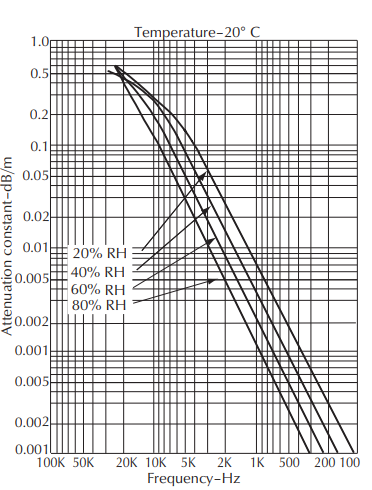
\includegraphics[width=%
0.50\textwidth]{assorbimento}
\caption{Tabella dei coefficenti di assorbimento dell'aria}
\label{fig:assorbimento}
\end{figure}

\subsubsection{Umidità}

Il livello di umidità del gas si riferisce alla presenza o meno di molecole d’acqua nel mezzo. La sua influenza non è tanto impattante per quanto riguarda la velocità dell’onda, ma sull’assorbimento acustico totale comportando un abbattimento di intensità a diverse frequenze.

\subsubsection{Fenomeni di Riflessione}

Le riflessioni sono alla base di ciò che chiamiamo riverbero.
Consistono nella riflessione di un’onda sonora sulle diverse superfici che 
circondano l’evento acustico, esse siano pareti oppure oggetti che si interpongono
nella propagazione dell’onda.

Affinché ci sia una riflessione, la superficie riflettente deve necessariamente essere
più larga di almeno $\frac{1}{4}$ della lunghezza d’onda.
Quando l’oggetto è più piccolo di questa soglia si ha una diffrazione, ovvero l’onda sonora curva attorno ad esso.

Un altro fenomeno, che possiamo considerare inverso alla riflessione, è \emph{l’assorbimento}.
L’assorbimento è dovuto alle proprietà del materiale che, appunto, al posto di riflettere l’onda assorbono parte dell’energia, trattenendola e restituendo un’onda smorzata.
Più un materiale è assorbente, più sarà rapido il decadimento dell’energia sonora nello spazio fino a tornare in una situazione di stabilità.
La condizione di stabilità sussiste infatti, quando la quantità di energia assorbita è la medesima dell’energia prodotta.

\subsubsection{Fenomeni di Rifrazione}

La rifrazione similmente alla riflessione si ha quando è il mezzo di trasmissione a subire delle variazioni, comportando dunque una differenza nella propagazione in atto. Queste variazioni possono essere, per esempio, temperatura, densità o direttamente un mezzo diverso, basti pensare ad un onda prodotta in aria che incontra una superficie d’acqua.

\section{Psicoacustica}

Altro aspetto da tenere in considerazione è il nostro sistema uditivo. In un sistema lineare in frequenza data in input una lista di frequenze, l’output conterrà le stesse, anche se magari dissimili in ampiezza e fase.
Il nostro apparato uditivo, infatti, a causa di secoli di evoluzione e cambiamenti ha sviluppato dei comportamenti che non lo rendono un sistema lineare, portando dunque a delle inesattezze dal punto di vista percettivo.
Ecco alcuni esempi di fenomeni di non linearità a cui siamo sottoposti:

\begin{itemize}
\item Distorsione armonica:
È la percezione di armoniche superiori di un tono puro. Questa distorsione può essere dovuta ad una pressione eccessiva dell’onda sul timpano;
\item Tono di combinazione:
Detto anche \textit{“terzo suono di Tartini”} è un effetto psicoacustico che comporta nella percezione di un terzo suono, nonostante in input i suoni siano stati solo 2.
La frequenza del tono ricostruito non sarebbe altro che la differenza tra i 2 toni di partenza
\item Curve isofoniche:
Il fenomeno delle curve isofoniche comporta una diversa percezione di ampiezza a per diverse frequenze ma aventi stesso SPL. Per fare un esempio una sinusoide da 1000 Hz a 110 Db SPL ha la stessa percezione di una sinusoide da 3000 Hz ma a 100 Db SPL (ballou - Handbook for Sound Engineers - 2008 - pag 43).
\end{itemize}
\begin{figure}
\centering
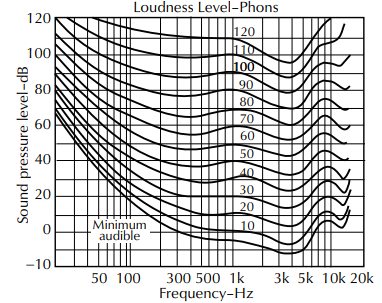
\includegraphics[width=%
0.50\textwidth]{isofoniche}
\caption{Grafico che mostra il comportamento delle curve isofoniche}
\label{fig:isofoniche}
\end{figure}
Questo è anche il motivo per il quale siamo più sensibili nella banda intorno ai 4 KHz, comportando dolore nell’ascoltatore se sottoposto a db elevati.
\subsubsection{Percezione della distanza}
Più interessante ai fini della tesi è la percezione della distanza, tema chiave nello studio degli spazi e della propagazione del suono.
È noto che, duplicata la distanza tra fonte sonora e ascoltatore, il SPL decade di 6 dB.
Nonostante questo, affinché abbiamo la percezione della duplicazione della distanza c’è bisogno della diminuzione di almeno 20 dB (j. Blauert spatial hearing).

Un elemento che però ci permette di comprendere quando una fonte è lontana è la sua composizione spettrale, infatti, a causa dell’assorbimento dell’aria (del mezzo per essere più precisi) le frequenze alte saranno assorbite maggiormente, comportando una presenza più elevata di basse frequenze.

Per questo, in modo tale da replicare distanza e vicinanza dalla fonte sonora, oltre a questi accorgimenti è da tenere in considerazione il rapporto tra suono diretto e riverberato.
In un ambiente reale infatti, è proprio il rapporto tra le due sorgenti a determinare dove e quanto è distante un evento sonoro.

\section{Spazio}
Come citato poc'anzi quando si parla di suono bisogna considerare quindi lo spazio e il mezzo in cui l'onda si propaga.
Possiamo classificare gli spazi in diverse categorie, le principali sono (Davis - Pag 178):
\begin{itemize}
\item Free Field:
È definito così uno spazio uniforme, libero da ostacoli che potrebbero produrre delle riflessioni o rifrazioni e non contaminato da sorgenti sonore estranee.
Esempi di questo tipo sono le sale anecoiche (senza eco),camere particolari il cui scopo è quello di ridurre al minimo le riflessioni delle onde, utili per eseguire test precisi su apparecchiature audio.
\item Reverberant field:
È uno spazio chiuso, con pochissimo assorbimento acustico, in cui la pressione sonora è uniforme in ogni punto e le onde si propagano allo stesso modo in tutte le direzioni.
Caratteristiche di questo tipo possiamo trovarle in luoghi come camere vuote o cavità.
\item Semireverberant Field:
È il tipo di spazio più comune che possiamo incontrare, nel quale l’energia è sia assorbita che riflessa. L’energia si muove in più direzioni ma è comunque percepibile il punto di origine della fonte di generazione dell’evento sonoro.
\end{itemize}
\subsection{Risposta all'impulso}
Al giorno d’oggi conosciamo una tecnica in grado di eseguire una fotografia delle caratteristiche acustiche in grado di descrivere come il suono si propaga da un punto di emissione ad un ricevitore. 

Parliamo di \textit{Risposta all’impulso} ovvero del modello fisico-matematico di un sistema lineare, non dipendente dal tempo, composto solo da un input ed un output (A.Farina - ROOM IMPULSE RESPONSES AS TEMPORAL AND SPATIAL FILTERS - 2006).

Le informazioni contenute sono sia relative al dominio del tempo, ad esempio riflessioni e ritardi nella propagazione che, relative al dominio della frequenza, comportando quindi modifiche dal punto di vista spettrale.

Il sistema utilizzato viene detto \textit{Black box} che, come detto in precedenza è composto da un singolo input ed un singolo output. All’interno di questa black box gli elementi che concorrono all’acquisizione dei dati matematici dello spazio che si vuole registrare sono:
\begin{itemize}
\item Un generatore di segnale: Tipicamente un pc;
\item Un amplificatore di segnale;
\item Un diffusore di segnale: il quale riproduce il segnale nello spazio in modo omnidirezionale;
\item Un ricevitore: un microfono anch’esso omnidirezionale, in quanto vogliamo escludere la direzionalità dallo studio.
\end{itemize}
Per misurare quindi la risposta all'impulso riproduciamo il segnale attraverso l’altoparlante nello spazio e contemporaneamente registriamo come, quel segnale, si propaga in quel determinato spazio e in quelle determinate condizioni, attraverso il microfono.

Il segnale originale consiste in uno sweep esponenziale il quale parte dalla frequenza $f_1$, termina a frequenza $f_2$ in $t$ secondi.

Il segnale riverberato conterrà al suo interno componenti armoniche non presenti nell’originale, che corrispondono alla risposta lineare in frequenza dello spazio.
Attraverso un processo di convoluzione, ampiamente spiegato e perfezionato dal prof. A Farina, siamo in grado di restituire la risposta all'impulso del sistema lineare.

È da tenere conto che però una singola registrazione non è in grado di descrivere tutto lo spazio. La risposta all’impulso, come già detto, è relativa soltanto al punto in cui è posizionato il ricevitore e soltanto per il punto da cui è emesso il suono. Per la mappatura dello spazio per restituire un'immagine fedele dello spazio sono necessarie numerose registrazioni. Come per una fotografia, maggiore è il numero di “pixel”, più definita sarà l’immagine. Per questo è un lavoro che, soprattutto per luoghi ampi, richiede moltissimo tempo e spesso si tende ad effettuare un numero di registrazioni non necessario a restituire un modello fedele.
\subsection{Storia dello studio degli spazi}
Storicamente, in ambito musicale, lo spazio è stato sempre presente ed essenziale durante le performance. Basti pensare agli auditorium greci, dove la conformazione permette sia un rinforzo in termini di ampiezza, ma anche una forte intelligibilità delle parole in modo tale da raggiungere chiaramente tutti i presenti.
Gli ascoltatori, posti ad un'angolazione di circa 120 gradi, ricevevano il suono diretto dall’oratore, seguito delle riflessioni provenienti sia dal pavimento dell’orchestra, che dal retro del palco, anche se con minor intensità.
\begin{figure}[h]
\centering
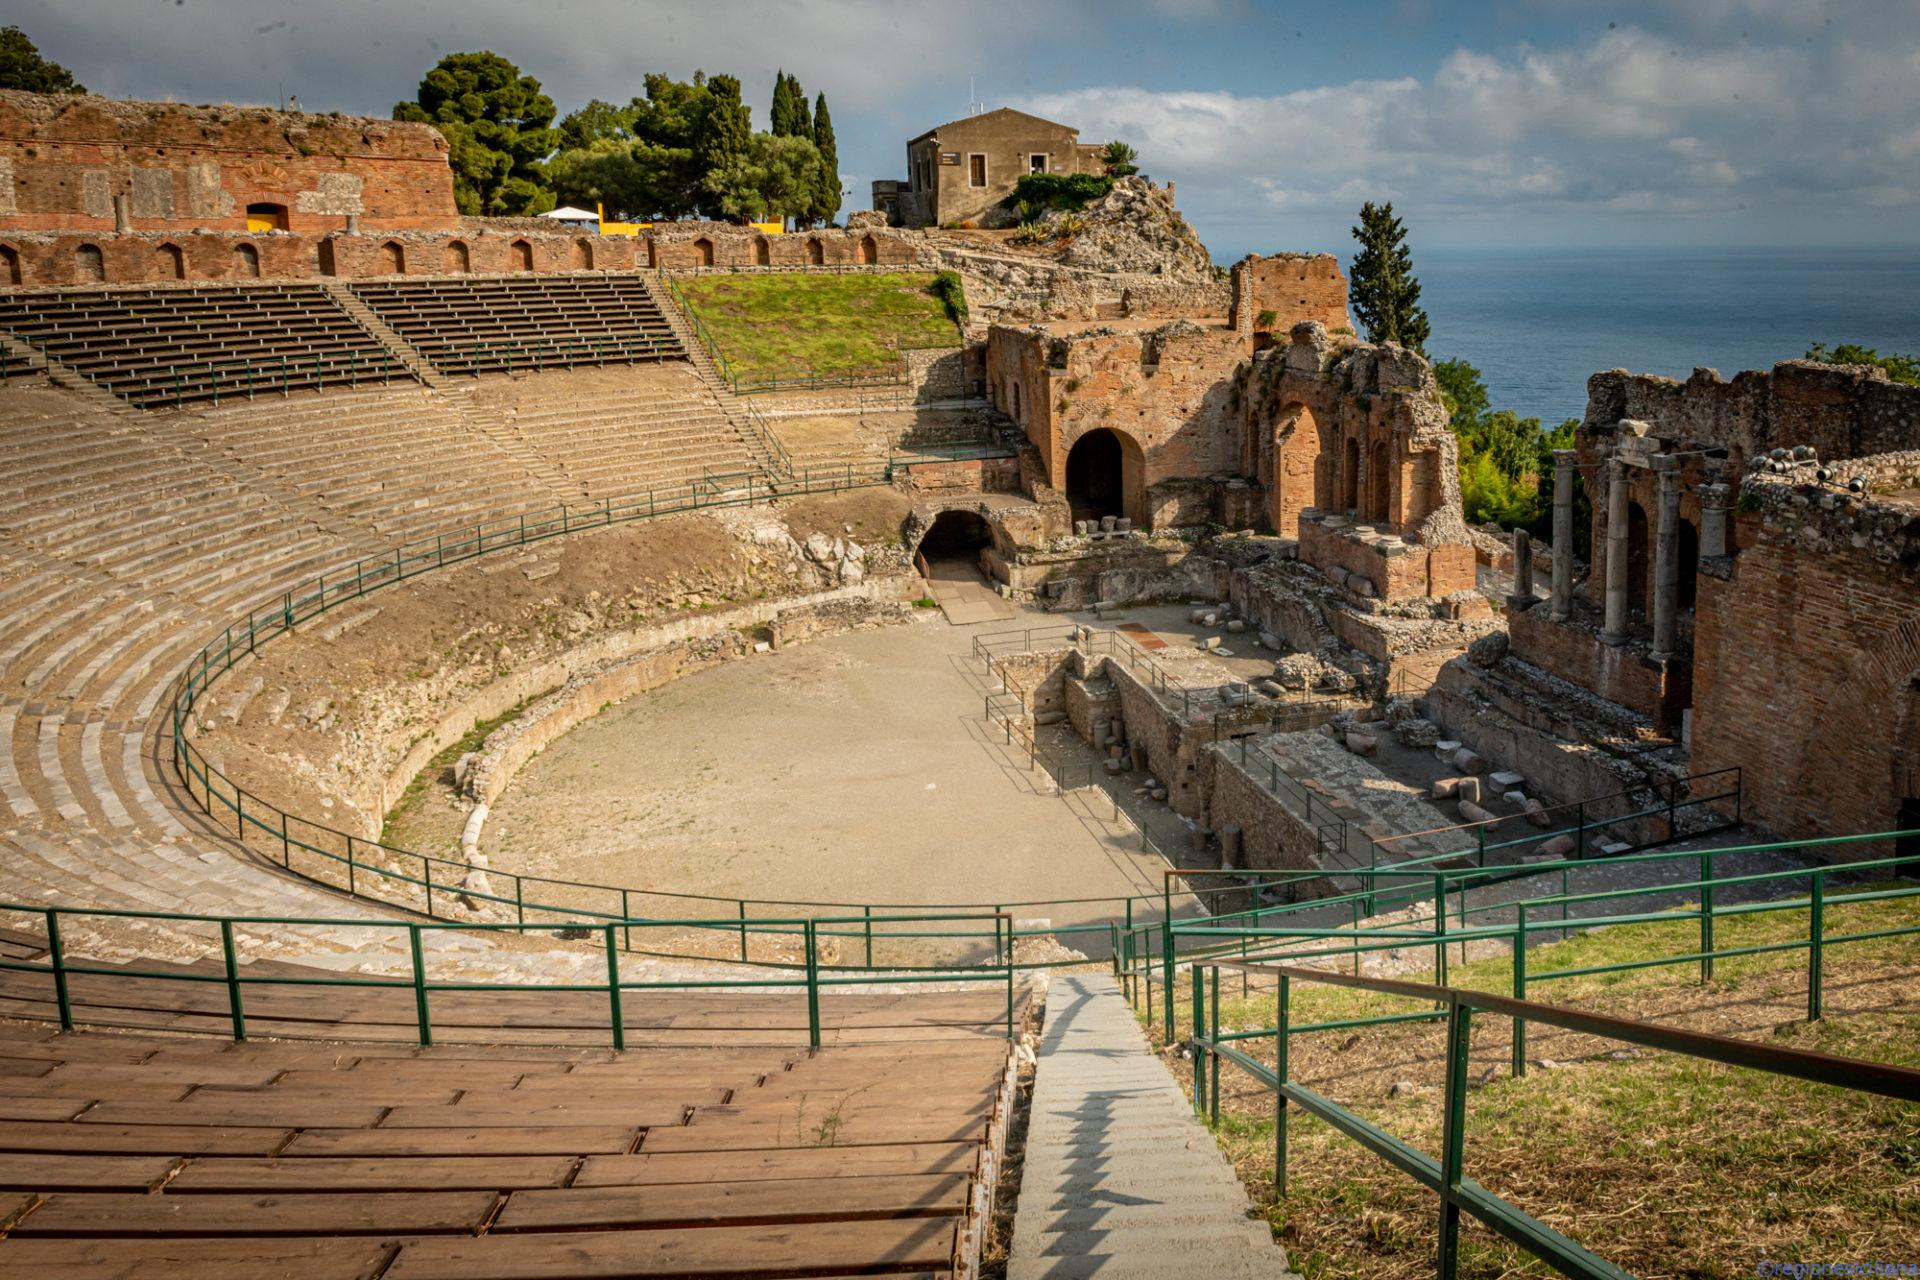
\includegraphics[width=%
0.50\textwidth]{teatrogreco}
\caption{Foto del teatro greco di Siracusa}
\label{fig:teatrogreco}
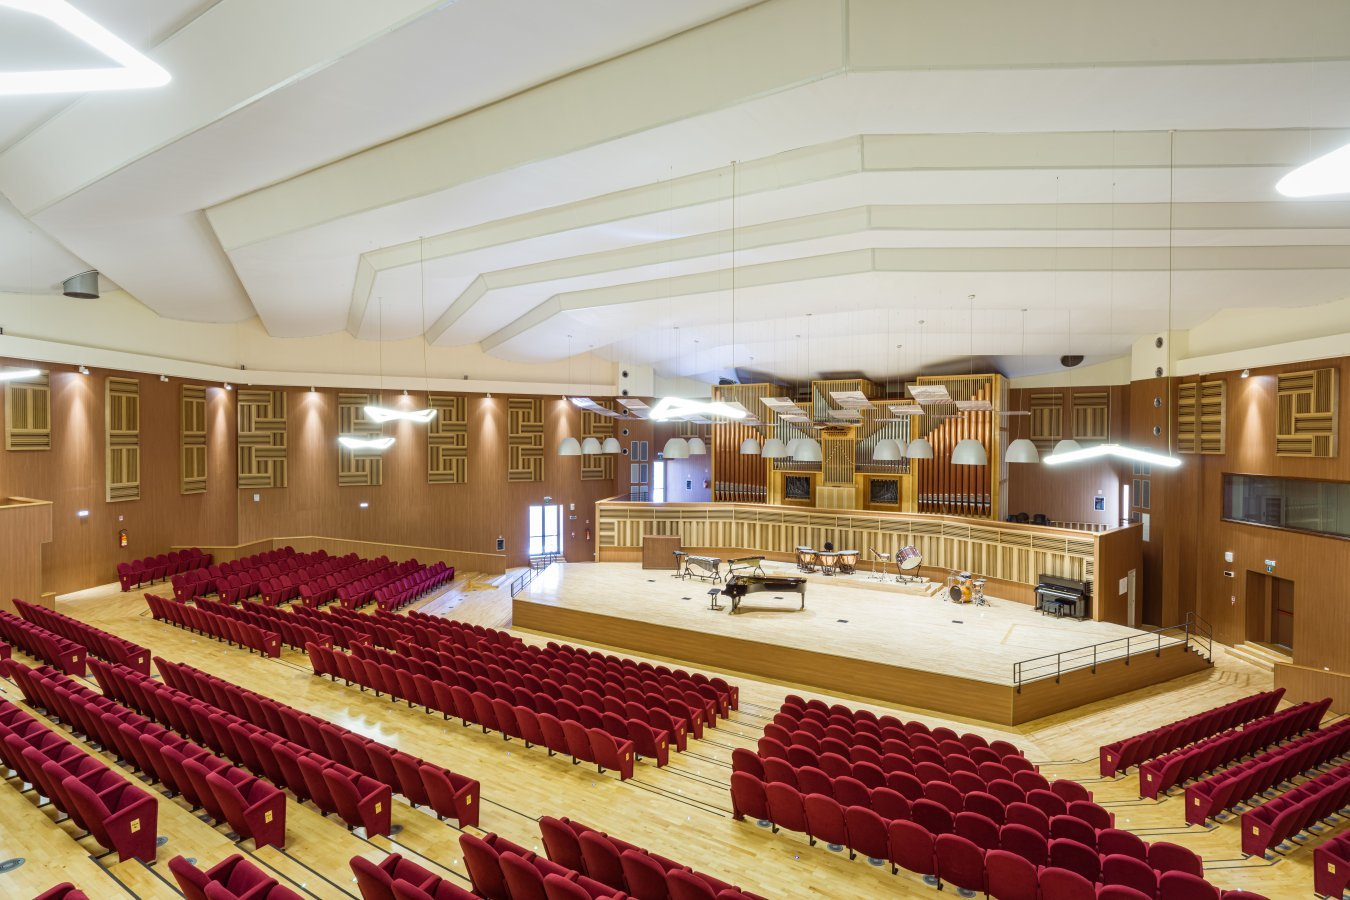
\includegraphics[width=%
0.50\textwidth]{auditorium}
\caption{Foto dell'auditorium Nino Rota del conservatorio di Bari}
\label{fig:auditorium}
\end{figure}
Il palco, inoltre, aveva un’ altezza compresa tra 1m e 3.6m, comportando una differenza nell’angolo di incidenza del suono diretto (Auditorium Acoustics and Architectural Design Di Michael Barron).
Infine, un altro accorgimento degli architetti greci, i quali avevano scoperto le proprietà di assorbimento, era il posizionamento tra le sedute di vasi contenenti ceneri, i quali avevano lo scopo di assorbire l’energia sonora che sarebbe stata riflessa indietro verso il palco.
\bigskip
Un’altro esempio in cui vediamo lo spazio come protagonista, è il caso degli organi, in cui il luogo è la vera e propria cassa armonica dello strumento.
L’acustica dell’organo è fortemente legata alla sua ubicazione, infatti, a differenza di altri strumenti musicali i quali possono essere spostati e trasportati, per l’organo non è possibile. Inoltre i luoghi provvisti di organo sono spesso molto riverberanti, come ad esempio le chiese e i teatri, e questo concorre alla definizione timbrica dello strumento
\begin{figure}[h]
\centering
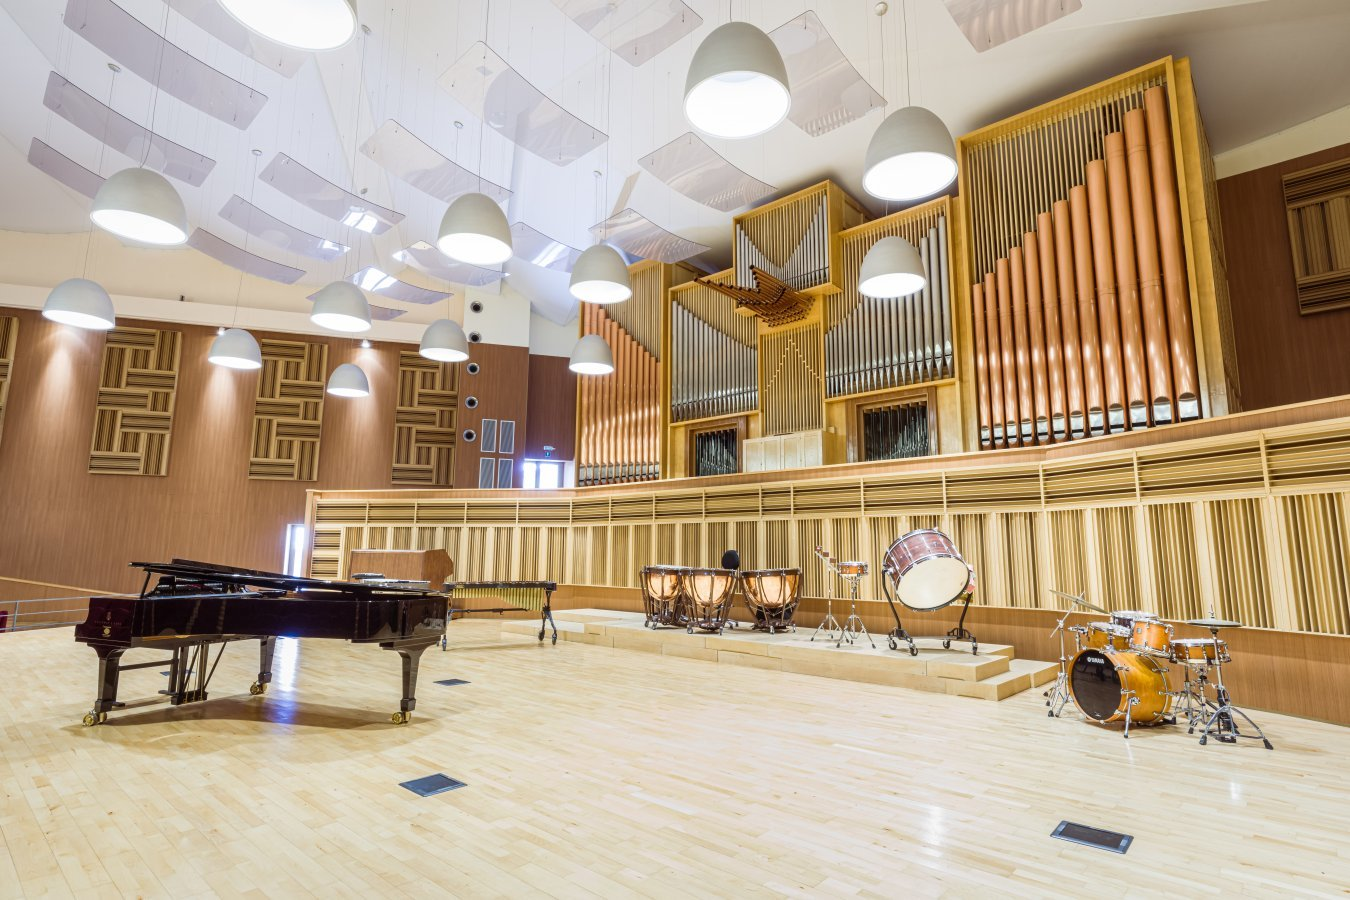
\includegraphics[width=%
0.50\textwidth]{organo}
\caption{Foto dell'organo presente nell'auditorium N.Rota}
\label{fig:organo}
\end{figure}
\subsubsection{Lo spazio come parametro}
Si è dovuto attendere però circa gli anni 60 affinchè lo spazio diventasse un vero e proprio parametro compositivo.

\emph{“Gesang der Jünglinge"} di Karlheinz Stockhausen è un’opera importantissima per l’epoca in cui è stata composta. Il brano, nato pentafonico e successivamente ridimensionato in quadrifonia, rappresenta l’avanguardia del serialismo integrale. Come accennato in precedenza, questo lavoro è il primo esempio in cui vediamo la gestione dello spazio come parametro compositivo, al pari di ampiezza, altezza e timbro.
Gli altoparlanti, disposti circolarmente attorno agli ascoltatori, creano uno spazio in cui immergersi permettendo complessi movimenti tra gli stessi.
Vengono infine introdotti termini quali “Intervallo spaziale” e “Accordi di spazio”.
\subsection{In conclusione}
% !TEX TS-program = pdflatex
% !TEX root = ../tesi.tex

%************************************************
\chapter{Filtri}
\label{chp:Filtri}
%************************************************

Questo capitolo affronta l'ampio mondo dei filtri, sui loro utilizzi, comportamenti e architetture, ponendo uno sguardo all'utilizzo dei ritardi nel loro design.

\section{Filtri}
Prima di proseguire con l’analisi del riverberatore, c’è bisogno di introdurre il concetto di filtro, oggetto essenziale  per la creazione di quest’ultimo.
Un filtro possiamo definirlo come un dispositivo o rete di dispositivi in grado di separare segnali complessi in base alla loro frequenza. Un filtro, come suggerisce il nome, filtra e permette ad alcune bande di frequenze di essere successivamente emesse oppure escluse dall’output finale. 
Alcune caratteristiche presenti nella maggior parte dei filtri sono:
\begin{itemize}
\item Banda Passante:
Banda di frequenze che passa attraverso un filtro e che subisce una perdita di meno di 3 dB;
\item Banda Stoppata:
Banda di frequenze che passa attraverso un filtro e che subisce una perdita di 3 db o più; 
\item Frequenza di Taglio
È la frequenza dove il filtro inizia ad eseguire modifiche al segnale, come abbattimenti o enfatizzazioni;
\item Ordine:
È una caratteristica definita dal numero di oggetti all’interno del filtro che concorrono al medesimo risultato, di solito inerenti a scopi di risposta in frequenza del filtro. Se tutti gli elementi sono eterogenei, per esempio passa basso o passa alto, l’attenuazione sarà di 6 db per ordine. Un filtro passa basso del quarto ordine avrà abbattimento di 24 db, ma un passa banda del medesimo ordine ne abbatterà soltanto 12.
\end{itemize}
\medskip
\subsection{Categorie di filtri}
In seguito a queste caratteristiche, passiamo ad eseguire brevi categorizzazioni di filtri in base alla loro componentistica e comportamenti.

Una prima categorizzazione che possiamo eseguire, riguarda la presenza o meno, di componenti che amplificano il segnale. Parliamo di:
\begin{itemize}
\item Filtri Passivi:
Sono filtri che non possiedono amplificatori di segnale, quindi il loro unico scopo è quello di attenuare ciò che li attraversa;
\item Filtri Attivi:
Al contrario, i filtri attivi hanno componenti che permettono l’amplificazione di determinate bande o dell’intero segnale, aggiungendo energia dove necessario.
\end{itemize}

Parliamo di \textbf{equalizzatore} per identificare un dispositivo il cui scopo è quello di sopperire a caratteristiche non gradite, riguardanti ampiezza, frequenza o fase, in modo tale da ricreare la risposta desiderata. Gli equalizzatori, per compiere ciò, sono costituiti da filtri, implementati per svolgere diversi tipi di modifiche.

\section{Funzione di trasferimento}
Prima di proseguire è necessario affrontare in questa sezione un concetto matematico che negli anni ha contribuito allo studio e alla creazione di filtri digitali grazie alla sua estrema versatilità, ovvero le funzioni di trasferimento.
 
In breve, una funzione di trasferimento è la trasformata della risposta all’impulso di un sistema LTI (Linear Time-Invariant) e riassume in sé le sue caratteristiche.

Si presenta nella seguente forma:
\begin{equation}
H(s)=\frac{\sum_{k=0}^K a_k s^k}{\sum_{n=0}^N a_n s^n}
\end{equation}

È definita tramite una funzione razionale fratta, ovvero una funzione costituita dal rapporto di due polinomi. Ognuno dei due polinomi individua un’equazione rispettivamente di $k$-mo e $n$-mo grado ovvero che ci saranno $k$ soluzioni per il polinomio al numeratore ed $n$ soluzioni per il polinomio al denominatore. Queste soluzioni saranno tutti i valori che rendono nulla la funzione: quelle che azzerano il numeratore si dicono \textbf{zeri} $(-zk)$, quelle che azzerano il denominatore si dicono \textbf{poli} $(-pn)$.

La forma fattorizzata della funzione di trasferimento è la seguente ed è utilizzata per il tracciamento dei grafici di risposta in frequenza dei filtri (detti diagrammi di bode)
\begin{equation}
H(s)=\frac{\prod_{k=1}^k (s+zk)}{\prod_{n=1}^n (s+pn)}
\end{equation}
\bigskip 
Semplificando il tutto e ricollegandoci all’argomento principale, è necessario comprendere che poli e zeri corrispondono alla frequenza di taglio del filtro che la funzione di trasferimento rappresenta.
\section{Tipologie di filtro}
Come detto in precedenza, i filtri si distinguono per via della loro architettura alla quale consegue un diverso comportamento. Ecco alcune tipologie di filtro, tra le più comuni:

\subsection{Low-Pass}
Permette l’attenuazione delle frequenze superiori alla frequenza di taglio.
La sua funzione di trasferimento è la seguente
\begin{equation}
H(s)=\frac{1}{1+st}
\end{equation}
dove con $st$ indichiamo la frequenza di taglio.

\begin{figure}[h]
\centering
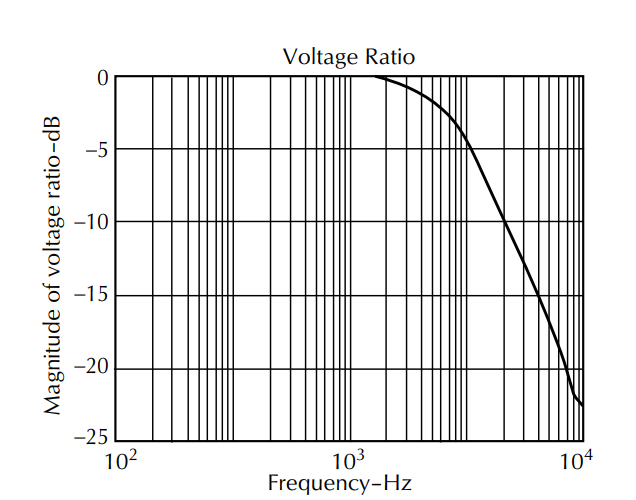
\includegraphics[width=%
0.50\textwidth]{lp}
\caption{Diagramma di Bode di un filtro passa basso \newline \scriptsize{ da D. Davis - Sound System Engineering - 2013}}
\label{fig:lp}
\end{figure}

\subsection{High-Pass}
Permette l’attenuazione delle frequenze inferiori alla frequenza di taglio.
La sua funzione di trasferimento è in figura \ref{fig:hp}

\begin{equation}
H(s)=\frac{st}{1+st}
\end{equation}

dove con $st$ indichiamo sempre la frequenza di taglio.
La risposta in frquenza ottenuta è la seguente
\begin{figure}[htp]
\centering
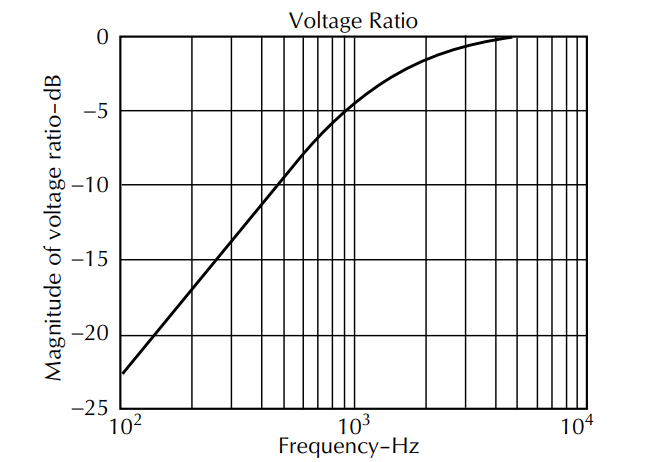
\includegraphics[width=%
0.50\textwidth]{hp}
\caption{Diagramma di Bode di un filtro passa alto}
\label{fig:hp}
\end{figure}

\subsection{Band-Pass}
Permette il passaggio solo ad una determinata banda di frequenze.
la sua funzione di trasferimento è la seguente
\begin{equation}
H(s)=\frac{(1+st_1)(1+st_4)}{(1+st_2)(1+st_3)}
\end{equation}
Considerando che $t_1>t_2>t3_>t_4$ e che il calcolo di poli e zeri risulta: $z_1=1/t_1$, $z_2=1/t_4$, $p1_=1/t_2$, $p_2=1/t_3$ \dots

La risposta in frquenza ottenuta è in figura \ref{fig:bp}
\begin{figure}[htp]
\centering
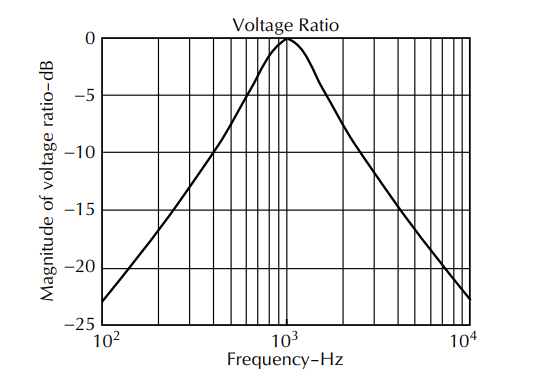
\includegraphics[width=%
0.50\textwidth]{bp}
\caption{Diagramma di Bode di un filtro passa banda}
\label{fig:bp}
\end{figure}


\section{Filtri Digitali}

Ovviamente tutto ciò che abbiamo visto fino a questo punto è puramente nel dominio continuo. Possiamo dunque procedere all’implementazione di tali modelli matematici in digitale. I filtri digitali utilizzano in larga scala algoritmi ricorsivi aventi al loro interno moltiplicazioni e addizioni, per i quali gli attuali strumenti informatici di cui disponiamo, sono ottimizzati. Definiamo 2 macro categorie di filtri digitali ovvero i cosiddetti filtri \textbf{FIR} e \textbf{IIR}.
\begin{itemize}
\item IIR: Infinite impulse response;
\item FIR: Finite impulse response.
\end{itemize}
Possiamo definire i filtri IIR come caratterizzati da una risposta all’impulso unitario non limitata (parlando di numero di campioni) e un’ampiezza tendente a zero.
Questo rende i filtri IIR molto simili alla loro controparte analogica (esistente nel tempo continuo).
Per quanto riguarda la loro composizione strutturale, notiamo generalmente una funzione di trasferimento costituita da un rapporto polinomiale, con poli e zeri. È esclusa una situazione in cui siano presenti soli zeri. Inoltre la costruzione di questi filtri prevede l’utilizzo di sistemi di feedback, e per questo, è risaputo che queste strutture hanno un comportamento instabile. 

Parlando di filtri FIR, invece, possiamo affermare che la loro risposta all’impulso unitario è composta da un numero finito di campioni e per questo non associabili a nessun modello analogico.
A differenza dei filtri IIR, i filtri FIR, presentano una funzione di trasferimento a soli zeri.
Possedere una risposta all’impulso unitario limitata comporta, inoltre, una stabilità nell'implementazione, ma di conseguenza una necessità di maggiore potenza di calcolo.
(Lindoro del Duca - Musica Digitale - pag 85)

\section{Delay e Utilizzo}
Il \emph{Delay} è il ritardo temporale imposto ad un evento sonoro. Il Delay può essere percepito soltanto se messo in relazione ad un altro segnale, ovvero, il suono stesso ma non ritardato.
Questo fenomeno si manifesta in due situazioni: quando, in un ambiente riverberante il suono diretto raggiunge l’ascoltatore prima delle sue riflessioni, oppure quando, un delay elettrico, è volontariamente inserito per pareggiare due sorgenti sonore e simulare un’ unica provenienza.

Il delay è inoltre un componente chiave nella costruzione dei filtri digitali.
Nel dominio digitale, infatti, i singoli campioni di una sequenza vengono sottoposti a numerose operazioni (implicando un processo di quantizzazione) producendo una seconda sequenza di risultati che comporranno il segnale filtrato. 
Le operazioni utilizzate sono: Somma, Prodotto e Delay (di un campione).
L’espressione che determina il comportamento del filtro è detta equazione differenza e, in base al numero di elementi di ritardo presenti, possiamo indicare l’ordine dell’equazione.

L’equazione differenza del primo ordine generale è definita secondo la seguente equazione:

\begin{equation}
Y(z)=A_0*x(z) + A_1*z^{-1}*x(z) + B_1*z^{-1}*y(z)
\end{equation}

L’equazione è scritta nel dominio z, con z detta frequenza complessa.
I valori di z che rendono rispettivamente nullo numeratore e denominatore vengono detti zeri e poli della funzione.

Tutte le equazioni differenza del primo ordine sono determinate dai coefficienti $A_0, A_1,B_1$.
Bisogna sempre considerare che un’equazione del primo ordine può descrivere solo un filtro passa basso o passa alto avente un’attenuazione di massimo 6 dB/ottava.

Partendo dall’equazione differenza, infine, possiamo ricavare la funzione di trasferimento $H(z)$ avente la seguente forma:

\begin{equation}
H(z)=\frac{(A_0 + A_1 * z^{-1})} {(1-B_1 * z^{-1})}
\end{equation}

% !TEX TS-program = pdflatex
% !TEX root = ../tesi.tex

%************************************************
\chapter{Storiografia dei Riverberi}
\label{chp:Storiografia dei Riverberi}
%************************************************

Questo capitolo affronta l'ambito fisico della produzione e dispersione dell'onda sonora
% !TEX TS-program = pdflatex
% !TEX root = ../tesi.tex

%************************************************
\chapter{Implementazione}
\label{chp:Implementazione}
%************************************************

In questo capitolo sarà presente l’analisi degli algoritmi che compongono il sistema riverberante creato. Gli algoritmi sono stati scritti nel linguaggio Faust sulla base delle ricerche svolte da Schroeder e Moorer e presentano le dovute modifiche che rispecchiano l’idea iniziale, vale a dire utilizzando parametri quali temperatura, pressione e tipologia del gas per variare la risposta del riverbero.

\section{Algoritmi di Schroeder}

I primi algoritmi sono stati creati partendo dalle soluzioni ottenute da Schroeder e utilizzati a scopo di test. L’obiettivo è stato quello di ricreare passo dopo passo le unità descritte nell’articolo Natural Sounding Artificial Reverberation. 

\subsection{Algoritmi fondamentali}

Partendo quindi dagli elementi fondamentali, abbiamo, come primo sistema il filtro Comb descritto in \ref{fig:dfl}.
\begin{code}
dfld(t, g) = ( + : de.delay(ma.SR,t-1))~(*(g)) : mem; //delay feed loop 
process = os.impulse : dfld(1000,.707);
\end{code}

Il codice presenta le variabili t e g che rappresentano rispettivamente il numero di campioni di ditardo e il moltiplicatore del feedback.
La funzione de.delay è utilizzata per il ritardo di un determinato numero di campioni.
Il simbolo \verb!~! permette l'utilizzo di una recursione, ovvero divide il segnale inviando una sua copia all'entrata del processo, creando \emph{feedback}
Il diagramma di questo codice è in figura \ref{fig:dflfaust}.

\bigskip

\begin{figure}[htp]
\centering
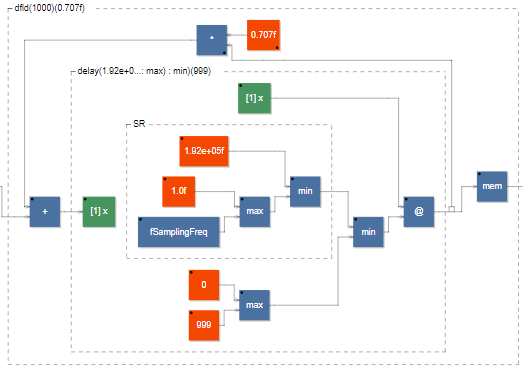
\includegraphics[width=%
0.80\textwidth]{dflfaust}
\caption{delay feedback loop}
\label{fig:dflfaust}
\end{figure}

Il secondo algoritmo derivato permette di realizzare un filtro All Pass, come quello descritto in figura \ref{fig:apf}

\begin{code}
apf(t,g) = _ <: *(-g) + (dfld(t,g)*(1-g^2));
process = os.impulse : apf(1,.71);
\end{code}

Il comportamento All Pass è dato dalla somma del segnale ritardato moltiplicato per $(1-g^2)$ e il segnale diretto moltiplicato per $-g$
Il diagramma di questo codice è in figura \ref{fig:apfaust}.

\begin{figure}[htp]
\centering
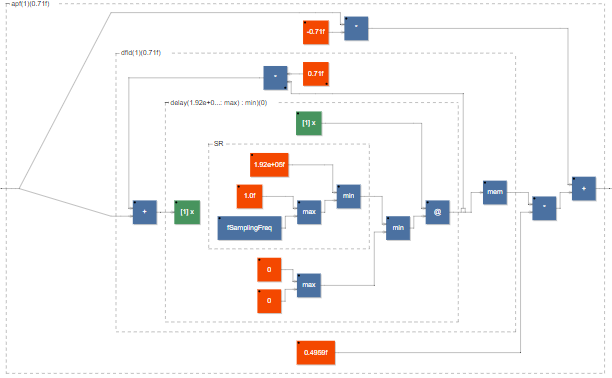
\includegraphics[width=%
0.90\textwidth]{apfaust}
\caption{All Pass}
\label{fig:apfaust}
\end{figure}

\subsection{Algoritmi derivati}

I prossimi algoritmi sono i successivi descritti da Schroeder. Presentano una serie di miglioramenti che auspicano ad una maggior naturalezza nella risposta del filtro. 
Come abbiamo visto in figura \ref{fig:apfmix}, creiamo un All Pass contenente un secondo All Pass e un delay al suo interno, per simulare il ritardo che intercorre tra il suono diretto e il suono riverberato.

\smallskip

il nuovo All Pass è dunque:
\begin{code}
dflda(t,g) =  (+ : de.delay(ma.SR,t-1) : apf(t,g))~ *(g) : mem;
\end{code}

Il suo diagramma lo troviamo in figura \ref{fig:dfldafaust}

\begin{figure}[htp]
\centering
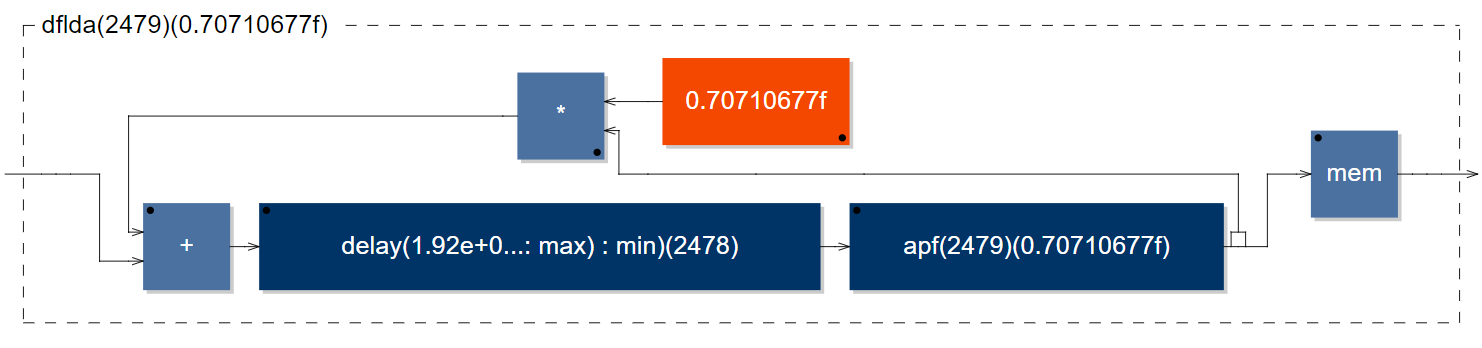
\includegraphics[width=%
0.90\textwidth]{dfldafaust}
\caption{Nuovo All Pass}
\label{fig:dfldafaust}
\end{figure}

Dato che abbiamo la necessità di missare il risultato del precedente filtro con il segnale diretto, creiamo un secondo ogetto che ci permette di farlo.

\begin{code}
apfn(t,g) = _ <: *(-g) + dflda(t,g) * (1-g^2);
\end{code}

\begin{figure}[htp]
\centering
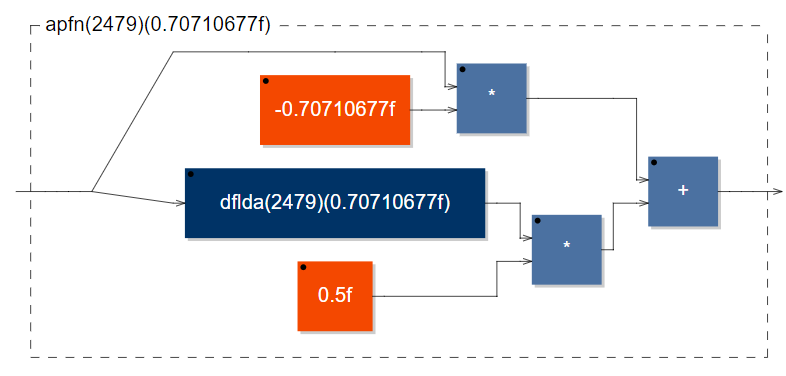
\includegraphics[width=%
0.70\textwidth]{apfmixfaust}
\caption{Nuovo All Pass con mix segnale diretto}
\label{fig:apfmixfaust}
\end{figure}

Il valore di g, inoltre, permette di decidere la quantità di segnale riverberato che vogliamo, come se fosse un pomello `'Dry/Wet''.

\subsection{Algoritmi Combinati}
Come già visto nel Capitolo 3, queste unità riverberanti non risultano particolaremente efficenti dal punto di vista della densità, se prese singolarmente, quindi il prossimo passo, come suggerito da Schroeder, è quello di crare delle reti di riverberatori combinando queste unità fondamentali.

\bigskip

Le due tipologie proposte consistono in una serie di All Pass connessi (figura \ref{fig:apfseq}), per la prima e, una serie di Comb connessi in cascata seguiti da 2 All Pass in serie, per la seconda.
Durante questa fase sono stati utilizzati numeri primi come valori dei ritardi in modo da evitare errori dovuti al campionamento.

L'algoritmo per la configurazione in serie risulta essere

\begin{code}
apfseq =  seq(i, 5, apf(ba.take(i+1, primet10),.7));
\end{code}

La lista ''primet10'' è stata caricata con i valori dei vari t. Come suggerito dall'autore, si è cercato di utilizzare numeri primi che mantenessero una relazione di $1/3$ l'uno dall'altro.
Il diagramma risultante è in figura \ref{fig:apfseqfaust}.

\begin{figure}[htp]
\centering
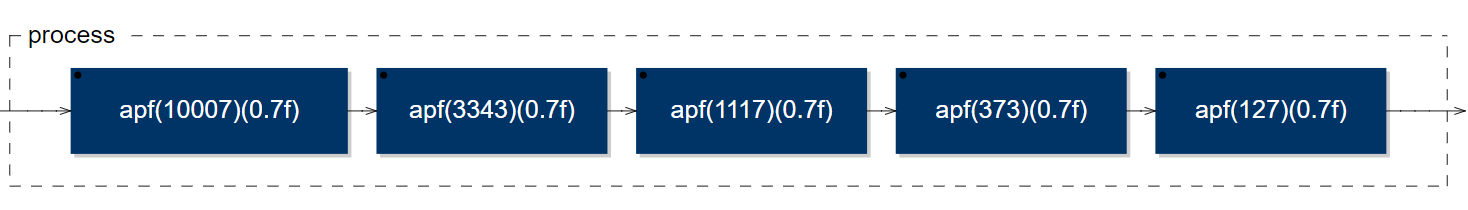
\includegraphics[width=%
0.90\textwidth]{apfseqfaust}
\caption{Sequenza di All Pass}
\label{fig:apfseqfaust}
\end{figure}

Il secondo algoritmo, per la configurazione `'Comb-All Pass'' vista in figura \ref{fig:comballpass}, è descritto nel seguente algoritmo

\begin{code}
reva((t,g,t1,g1),g2) = _<:_+(
    par(i,6, dflda(ba.take(i+1, t),G*ba.take(i+1,g))) :> 
    seq(i, 2, apfn(ba.take(4-i, t1),G*ba.take(i+1,g1))))*(g2);
process = _ : reva((primetc1,combg1,primetc2,combg2),G);
\end{code}

`'par'' e `'rev'' sono rispettivamente, composizione parallela e composizione sequenziale e ci permettono di creare una cascata di 6 Comb seguita da una sequenza di 2 All Pass. 

Il risultato è in figura \ref{fig:comballpassfaust}.

\begin{figure}[htp]
\centering
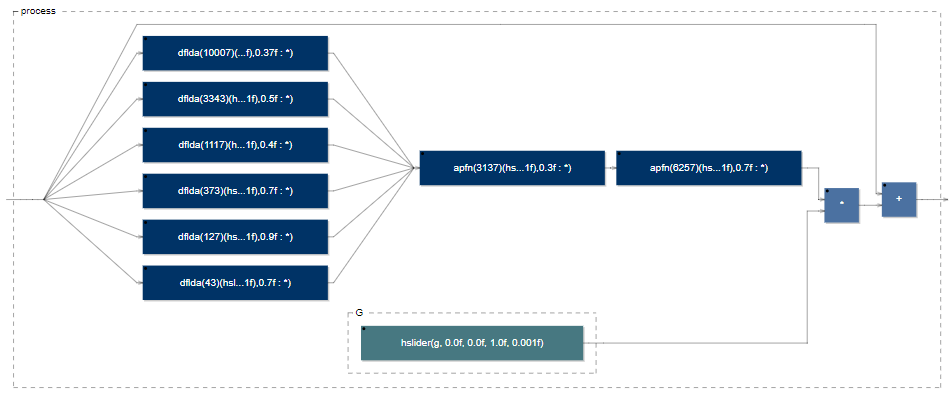
\includegraphics[width=%
1.2\textwidth]{comballpassfaust}
\caption{Algoritmo Comb-All Pass}
\label{fig:comballpassfaust}
\end{figure}
\clearpage
% !TEX TS-program = pdflatex
% !TEX root = ../tesi.tex

%************************************************
\chapter{Conclusione}
\label{chp:Conclusione}
%************************************************


% !TEX TS-program = pdflatex
% !TEX root = ../tesi.tex

%*******************************************************
% Bibliography
%*******************************************************
\nocite{*}
\printbibliography

\end{document}
